\documentclass[11pt, letterpaper, twoside, final]{article}
\usepackage{risk_price_inference}
\addbibresource{riskpriceinference.bib}

\author{Xu Cheng\thanks{University of Pennsylvania, The Ronald O. Perlman Center for Political Science and
    Economics, 133 South 36th Street, Philadelphia, PA 19104, \href{mailto:xucheng@upenn.edu}{xucheng@upenn.edu}}
    \and 
    Eric Renault\thanks{Brown University, Department of Economics -- Box B, 64 Waterman Street, Providence, RI
    02912, \href{mailto:eric_renault@brown.edu}{eric\_renault@brown.edu}}
    \and 
    Paul Sangrey\thanks{University of Pennsylvania, The Ronald O. Perlman Center for Political Science and
    Economics, 133 South 36th Street, Philadelphia, PA 19104, \href{mailto:paul@sangrey.io}{paul@sangrey.io}}}
    
\title{Inference for Risk Prices using Equity Data}

\date{\today}

\begin{document}

\begin{titlepage}


    \maketitle
    \thispagestyle{empty}
    \addtocounter{page}{-1}

    \begin{abstract} \singlespacing \noindent 
        The risk-return trade off is a central question in modern asset pricing. 
        Even though the theoretical literature cohesively argues there should be a strong positive correlation
        between expected returns and volatility, empirically measuring it has proven difficult. 
        In addition, the option pricing literature shows that volatility enters as its own risk factor, not just
        as a predictor of returns.
        Even obtaining point estimates of these risk prices in the presence of contemporaneous correlation between
        returns and volatility, the  volatility feedback effect, has proven delicate.
        We develop methods to provide  valid confidence intervals for the price of volatility and equity risk from
        equity data directly that account for this weak identification of the various parameters. 
        We do this by adapting the results in weak identification literature that uses drifting sequences in order
        to be robust to the data's identification strength. 
    \end{abstract}

    \jelcodes{C12, C14, C38,  C58, G12}

    \keywords{identification, robust inference, stochastic volatility, leverage, equity risk premium, volatility
    risk premium, risk price, confidence set, asymptotic size}

\end{titlepage}

\phantomsection
\addcontentsline{toc}{section}{Introduction}

Modern finance is all about the risk return trade offs that investors face and how to optimally respond to them. 
In particular, the central question of asset pricing is what drives expected returns.
Standard economic theory predicts you must compensate investors with higher expected returns when they face more
risk.
In other words, we would expect a positive relationship between the mean and volatility of returns.
In fact, in \gentextcites{sharpe1964capital,lintner1965security} capital asset pricing model (CAPM) the expected
return varies proportionally with the volatility. 
In other words, we have a constant price of volatility risk and expected returns are perfectly correlated with
volatility.
Even in more complicated models such as the long-run risk model and rare disasters models find a very close
relationship between variance and mean of returns \parencite{bansal2014volatility, wachter2013can}.

Consequently, an important empirical question is what is the precise magnitude of this relationship.
However, unlike the consensus in the theoretical literature, the empirical literature has found pinning down this
relationship quite difficult.
Not only has its magnitude proven difficult to determine, but various estimates even differ in sign,
\parencite{lettau2010measuring}, .

The empirical literature, which we examine in more detail in the literature review, has focused on point estimates
of this magnitude. 
However, if individual investors are ambiguity averse as in \textcite{hansen2001robust, jiu2012ambiguity}, they
will care not just about how the representative investor prices volatility but also their uncertainty regarding
this estimate. 
Furthermore, when economists calibrate models, they need to know how precisely the data determine the parameters
they are calibrating.
If the need to alter the parameter value slightly in order to make their model perform well, are they bringing in
more restrictions or data to more precisely determine the parameter of interest or are they using a value that the
data tell us is incorrect?

Clearly, as obtaining precise believable point estimates of the price of volatility risk has proven quite
difficult, we should expect doing valid inference to be even more delicate.
To the best of our knowledge, this is the first paper to directly tackle this question.
Various authors report confidence intervals as well as their point estimates.
However, they do not take into account the weak identification that makes getting the point estimate difficult in
computing these estimates.

Why is it that measuring this price is so difficult when the theoretical literature is so cohesive?
Econometrically, it is because the volatility price is weakly identified, as in \textcite{andrews2012estimation},
in that the strength of the identification of the price depends upon the value of other parameters. 
This obviously begs the question --- what are these parameters? 

To estimate the risk prices, there are three different phenomena that must be distinguished.
First, the econometrician must disentangle the volatility feedback effect (leverage) which is a contemporaneous
relationship between the volatility and returns from the risk premium, which is a relationship between volatility
and expected returns. 
It is not a contemporaneous relationship, but rather a predictable one. 

Second, and just as important.
In the papers estimating the volatility expected-return relationship such as
\textcite{brandt2004relationship,lettau2010measuring} are implicitly using a one-factor model where volatility
is that factor.
However, the option pricing literature, such as  \textcite{christoffersen2013capturing}, has argued that in order
to match the option pricing data we need to include another factor.
In other there are two sources of risk that the investors face: what returns will do and what the volatility
will do.
One can view the loading on the equity risk to itself be a function of the volatility.
The econometrician can rewrite this as a two factor model with equity and volatility risk up to higher order
terms.
Since, the econometrician must disentangle these two effects, their ability to do this will depend upon various
other parameters.
As mentioned in the introduction,in CAPM we only have factor, and so clearly we cannot disentangle them.
However, most models of interest to economists nest CAPM as a special case. 
Consequently, for certain values of the parameters, the model has only one factor. 
This directly implies that we cannot separately identify the two risks for some values of the other parameters.
More generally, the identification strength of the risk prices depends upon the other parameters.
The weak identification literature shows that in these scenarios, the finite-sample distributions of the estimates
are highly nonstandard, and the usual asymptotic approximations do not perform well.


Hopefully, the reader has a high-level understanding of the issue in at hand, and why simple econometric
procedures does not provide a useful guide to the true uncertainty regarding the parameters.
The obvious next step is considering how we need to do this in practice.
Since the contribution of this paper is in terms of methodology and empirical results, we will take a model from
the literature that has the various components, instead of developing our own asset or option pricing model.
In particular, we take the model from \textcite{khrapov2016affine} and use it to estimate the relevant parameters. 

This model has a few nice features. 
First, it has both equity and volatility prices and a leverage effect. 
As such, it is the natural discrete time analogue of the \textcite{heston1993closedform} option pricing model. 
It has an exponentially affine stochastic discount factor  and shares with \textcite{heston1993closedform} the
advantage of having a structure preserving change of measure between the physical and risk-neutral models.
By doing our analysis in discrete-time we are able to more directly compare our results to risk-premia estimates
outside of the option pricing literature and the jumps in high-frequency innovations will not dramatically affect
our results.  
If we were to use a diffusion process in continuous time, we would be severely counterfactually constraining the
higher-order  moments of the process in way that would likely bias our inference. 

As far as estimation is concerned, we follow \textcite{khrapov2016affine} in using a finite version of spectral
General Method of Moments (GMM).
Effectively, we take some moments implied by the characteristic function of returns and use them in a standard GMM
setup.
The data we use are the bivariate series $\begin{pmatrix} r_{t+1}, \sigma^2_{t+1} \end{pmatrix}$.
$r_{t+1}$ is the daily return on some asset, and we use its associated realized volatility for $\sigma^2_{t+1}$.
We go into further detail in \cref{sec:data} regarding how we obtained it, the time-span covered, and so on.

\section{Literature Review}\label{sec:lit_review}


\section{The Model}\label{sec:model}

\addtocounter{subsection}{1}

We estimate the prices of some factors using moment conditions derived from an option pricing model. 
As is standard in that literature, we will do  this by specifying the physical and risk-neutral measures and their
relationship, i.e.\@ the stochastic discount factor or pricing kernel.
Let $\F_t$ be the representative investor's information set at time $t$, and $P_t$ be the price on the asset in
question, with associated return $r_{t+1}$ and volatility  $\sigma^2_{t+1}$.

Given $\F_{t}$, the vector $\left( r_{t+1},  \sigma^2_{t+1}\right)$ is drawn from some process --- $\PP$ --- the
physical measure. 
We can further define the risk neutral measure --- $\QQ$ ---  as the process that makes $P_t$ a martingale, i.e.\@
the following holds. 
The advantage of defining $\QQ$ is that for some payoff function --- $f$  -- that is a function of future return
--- $r_{t+1}$ and volatility $\sigma^2_{t+1}$ and potentially depends upon the current information available --
$\F_t$, we can price this payoff as its expectation with respect to $\QQ$.
In other  words, the price of $f(r_{t+1}, \sigma^2_{t+1}, \F_t)$ satisfies for all $t$ and for all $f$.
This is useful because we can choose $f$ to make our estimation convenient.

\begin{equation}
    P_t(f) = \E_{\QQ}\left[ f\left(r_{t+1}, \sigma^2_{t+1}, \F_{t}\right)  \mvert \F_{t}\right]
\end{equation}

Since $P_t(f), r_{t+1}$ and $\sigma_t^2$ are observable, if we specify a model for $\F_t$ in terms of observable
(to the econometrician) variables, this provides a moment condition that we can use. 
However, this condition does not identify everything we wish to estimate, in particular it does not identify the
risk prices. 


To see this, we complete the model by defining the stochastic discount factor --- $M_{t, t+1}$ --- as the
Radon-Nikodym derivative between the $\PP$ and $\QQ$ measures. 
No arbitrage guarantees that this will exist, \parencite{harrison1978martingales}.
Since risk prices arise from investors' demand for compensation to hold risk, i.e.\@ their risk-aversion, here is
where they show up in the $\QQ$ measure. 
(We collect the parameter of interest into a vector --- $\eta$.)


\begin{defn}{Asset Pricing Moments}
    \begin{equation}
        P_t(f)  = \E_{\QQ} \left[f\left(r_{t+1}, \sigma^2_{t+1} , \F_t\right) \mvert \F_t \right] =
        \E_{\PP}\left[M_{t,t+1}(\eta)f\left(r_{t+1}, \sigma^2_{t+1}, \F_t\right) \mvert \F_t \right] 
    \end{equation}
\end{defn}

\subsection{Dynamics}\label{sec:dynamics}

To specify the model we must specify what the $\PP$ and $\QQ$ measures are and what $M_{t, t+1}(\eta)$ is.
We start by specifying the $\PP$ measure.

Following \textcite{khrapov2016affine}, we assume that the variables are first-order Markov and there is no
Granger causality from return to the volatility and that returns are serially independent given the volatility
path.
In other words, the volatility drives all of the dynamics of the process.
Note, we do allow $\sigma^2_{t+1}$ and $r_{t+1}$ to be contemporaneously correlated, which they are in the data. 

We construct the following conditional Laplace transforms as follows.
This is well-defined because we can define the true Laplace transform as the expectation of a specific function,
and then integrate out all of the unknown variables using their marginal distributions.
Hence, we can represent out model under the physical  as follows for some functions $a_{\PP}, b_{\PP},
\alpha_{\PP}, \beta_{\PP}$, and $\gamma_{\PP}$ for all $u$ in its domain.

\begin{restatable}[The Limited Information Model under the Physical Measure]{defn}{physicalMeasureModel}
    \label{defn:physical_model}
    \begin{align}
        \E_{\PP} \left[\exp(-u \sigma^2_{t+1}) \mvert \sigma^2_t \right] &= \exp\left( - a_{\PP}(u) \sigma^2_t -
        b_{\PP}(u) \right) \\
        \E_{\PP}\left[\exp(-u r_{t+1}) \mvert \sigma^2_t,  \sigma^2_{t+1}\right] &= \exp\left(- \alpha_{\PP}(u)
        \sigma^2_{t+1} - \beta_{\PP}(u)\sigma^2_t - \gamma_{\PP}(u) \right) 
    \end{align}
\end{restatable}

The difficult part moving forward is that we are identifying risk prices, which are  parameters of the stochastic
discount factor (SDF), but since we only observe equity data, we only observe the physical measure.
Consequently, we need to solve for the risk-prices as a function of the parameters governing the physical measure
an then invert this mapping.
In other words, we have some structural parameters --- the risk prices --- and we need to relate them to the
reduced form parameters --- the physical measure parameters.
We will do this by parameterizing the physical measure and the stochastic discount factor in terms of the first
few moments.
If higher moments, such as skewness and kurtosis are also priced factors, as in \textcites{harvey2000conditional,
conrad2012exante, chang2013market},  and we used higher sample moments as well to determine the price of our
risk-factors our resulting estimates would be biased, likely substantially so. 

As discussed in the introduction, this identification strategy is rather fragile.
Consequently, we need to take this weak identification into account when we construct the confidence sets.
We will do this by first deriving the joint distributions of the return and volatility in terms of the physical
measure parameters.
This is not trivial because we only modeled the conditional distribution of the $\left. r_{t+1} \mvert \sigma^2_{t},
\sigma^2_{t+1} \right.$  and $\sigma^2_{t+1}$ is not known at time $t$, and so we need to solve for it.


\subsection{Parameterizing the Physical Measure Dynamics}

The model in \cref{defn:physical_model} is parameterized using the functions mentioned, and at this level of
generality is fully nonparametric. 
We now derive the moment conditions that govern the physical measure. 
Note, by the physical-measure functions satisfy the following constraint by definition.

\begin{equation}
    a_{\PP}(0) = b_{\PP}(0) = \alpha_{\PP}(0) = \beta_{\PP}(0) = \gamma_{\PP}(0) 
\end{equation}

We can differentiate the Laplace transform at zero to compute the moments.
The logarithm of the Laplace transform above is a conditional cumulant generating function.
Since, we are only using the mean and variance, we can differentiate this function  and evaluate the
resultant function at zero to construct formulas for these moments.

We start by computing $\E_{\PP}\left[\sigma^2_{t+1} \mvert \F_t\right]$ and $\Var_{\PP}\left[\sigma^2_{t+1} \mvert
\F_t\right]$


\begin{align}
    \E_{\PP}\left[\sigma^2_{t+1} \mvert \sigma^2_t \right]  &= a_{\PP}'(0) \sigma^2_t  + b_{\PP}'(0) \\
    \Var_{\PP}\left[\sigma^2_{t+1} \mvert \sigma^2_t \right]  &= -a_{\PP}''(0) \sigma^2_t  - b_{\PP}''(0) 
\end{align}

To simplify the exposition, we will reparameterize these equations. 
Essentially, we will give these derivatives names.

\begin{defn}{Volatility Dynamics Parameters}
    \label{defn:vol_dynamics_params}
    \begin{align}
        \rho &\coloneqq a_{\PP}'(0) \in (0,1) \\
        c &\coloneqq - \frac{a_{\PP}''(0)}{2 a_{\PP}'(0)} > 0 \\
        \delta &\coloneqq -2 \frac{a_{\PP}'(0) b_{\PP}'(0)}{a_{\PP}''(0)} > 0 \\
        \omega &\coloneqq -4 \frac{b_{\PP}''(0) [a_{\PP}'(0)]^2}{[a_{\PP}''(0)]^2}
    \end{align}
\end{defn}

To interpret these factors, can derive a series of moments. 
$\rho$ is a persistence parameter.
$c$ is a scaling parameter.
We will also assume that the unconditional mean of $\sigma^2_t$ agrees with that of $\sigma^2_{t+1}$, and so we
can use the law of iterated expectation and the law of total variance to determine the moments.


\begin{align}
    \E_{\PP}\left[\sigma^2_{t+1} \mvert \sigma^2_t \right]  &= \rho \sigma^2_t  + c \delta\\
%
    \E_{\PP}\left[\sigma^2_{t+1}\right]  &= \frac{c \delta}{1 - \rho} \\
%
    \Var_{\PP}\left[\sigma^2_{t+1} \mvert \sigma^2_t \right]  &=  2 c \sigma^2_t  + c^2 \omega \\
%
    \Var_{\PP}\left[\sigma^2_{t+1} \right]  &=  \frac{c^2}{1- \rho^2} \left(\frac{2 \rho \delta}{1 - \rho}  + \omega
        \right) 
\end{align}

Clearly, we can identify all four of these parameters from the volatility data as long as the parameters are in
the interior of their domains.

We then turn to computing the moments of the return distribution. 
The first step is to compute the moments of the conditional distributions of $\left. r_{t+1} \mvert
    \sigma^2_{t+1}, \sigma^2_t \right.$.
As we did above, we can compute the conditional moments by evaluating the derivative the log-cumulant function at
zero.

\begin{align}
    \E_{\PP}\left[r_{t+1} \mvert \sigma^2_t, \sigma^2_{t+1}\right]  &= \alpha_{\PP}'(0) \sigma^2_{t+1}  +
    \beta_{\PP}'(0) \sigma^2_t + \gamma_{\PP}'(0) \\
    \Var_{\PP}\left[r_{t+1} \mvert \sigma^2_t, \sigma^2_{t+1}\right]  &= -\alpha_{\PP}''(0) \sigma^2_{t+1}  -
    \beta_{\PP}''(0) \sigma^2_t - \gamma_{\PP}''(0)
    \label{eqn:rtn_cond_vol}
\end{align}


Before we move to computing the moments of $\left. r_{t+1} \mvert \F_t \right.$, it is useful to simplify the
notation slightly.
We are using realized volatility  as our data for $\sigma^2_{t+1}$, and realized volatility is an
estimator for the realized variance of the martingale part of the process.
Consequently, $\Var_{\PP}\left(r_{t+1} \mvert \sigma^2_t, \sigma^2_{t+1}\right) \leq \sigma^2_{t+1}$.
Since the three second derivatives \cref{eqn:rtn_cond_vol} are constant, this implies that $\beta_{\PP}''(0)$ and
$\gamma_{\PP}''(0)$ both be non-positive for this to hold.
They cannot be negative or the conditional variance would be negative for small enough realizations of
$\sigma^2_{t+1}$.
In other words, we have the following equation.

\begin{equation}
    \Var_{\PP}\left[r_{t+1} \mvert \sigma^2_t, \sigma^2_{t+1}\right]  = -\alpha_{\PP}''(0) \sigma^2_{t+1} 
\end{equation}

I now introduce some notation to simplify the expression we have here.

\begin{align}
    \phi &\coloneqq \sqrt{1 - \abs{\alpha_{\PP}''(0)}} \\
    \psi &\coloneqq \alpha_{\PP}'(0)
\end{align}

We can then use the law of total variance to compute $\Var_{\PP}\left[r_{t+1} \mvert \F_t\right]$ and the law of
iterated expectations to compute $\E\left[r_{t+1} \mvert \F_t \right]$.

\begin{align}
    \label{eqn:lie_expected_rtn}
    \E_{\PP}\left[r_{t+1} \mvert \F_t\right] &= \psi \E\left[\sigma^2_{t+1} \mvert \F_t\right]  + \beta_{\PP}'(0)
    \sigma^2_t + \gamma_{\PP}'(0)  \\
%
    \label{eqn:ltv_rtn_variance}
    \Var_{\PP}\left[r_{t+1} \mvert \sigma^2_t\right]  &= (1 - \phi^2) \E \left[\sigma^2_{t+1} \mvert \sigma^2_t
    \right] + \psi^2 \Var_{\PP}\left[\sigma^2_{t+1} \mvert \sigma^2_t \right] 
\end{align}

In the next section we reparameterize \cref{eqn:lie_expected_rtn} in terms of risk prices.
This is natural because in the risk-neutral distribution this expectation equals zero, except for possibly $\psi$,
which can contain a Jensen type effect, which we will explain in detail later.
Consequently, the deviations from zero in the physical expectations reflect risk compensation. 


\subsection{The Stochastic Discount Factor}\label{sec:deriving_sdf_functions}

Since the Laplace transform for $r_{t+1}$  is exponentially affine under both $\PP$ and $\QQ$, the measure change
between them is also exponentially affine.
If we let $\pi$ be the price of volatility risk and $\theta$ be the price of equity risk, we can write down the
change of measure as follows.
We let $r_{f,t}$ be the risk-free rate.
It deterministically discounts the prices but plays no further role in the analysis.


\begin{defn}{The Stochastic Discount Factor}
    \begin{equation}
        M_{t,t+1}(\pi, \theta) = \exp\left(-r_{f,t}\right) \exp\left(m_{0}(\pi, \theta) + m_1(\pi, \theta)
        \sigma_t^2 - \pi \sigma^2_{t+1} - \theta r_{t+1}\right) 
    \end{equation}
\end{defn}


Before we show how the risk prices $\pi, \theta$ show up in the equations above, we will introduce some parameters
that govern the dynamics of the volatility process.
Since the SDF must integrate to $1$ once we discount using the risk-free rate $r_{f,t}$\, we have the following
restrictions.


\begin{gather}
    \E_{\PP}\left[\exp\left(m_0(\theta, \pi) + m_1(\theta, \pi) \sigma^2_t - \pi \sigma^2_{t+1} - \theta r_{t+1}
    \right) \mvert \F_t \right] = 1 \\
    \intertext{By the law of iterated expectations.}
    \E_{\PP}\left[ \E_{\PP}\left[\exp\left(m_0(\theta, \pi) + m_1(\theta, \pi) \sigma^2_t - \pi \sigma^2_{t+1}\right)
        \exp\left( - \theta r_{t+1}\right) \mvert \F_t, \sigma^2_{t+1} \right]\right] = 1 \\
    \intertext{The second term is the Laplace transform of $r_{t+1}$.}
    \E_{\PP}\left[\exp\left(m_0(\theta, \pi) + m_1(\theta, \pi) \sigma^2_t - \pi \sigma^2_{t+1} \right)
        \exp(-\alpha_{\PP}(\theta) \sigma^2_{t+1} - \beta_{\PP}(\theta) \sigma^2_{t} - \gamma_{\PP}(\theta_2)
        \mvert \F_t \right] = 1 \\
    \intertext{Reorganizing terms.}
    \E_{\PP}\left[\exp\left(m_0(\theta, \pi) + m_1(\theta, \pi) \sigma^2_t - \beta_{\PP}(\theta) \sigma^2_{t} -
        \gamma_{\PP}(\theta_2) \right) \exp(-\left(\pi + \alpha_{\PP}(\theta)\right) \sigma^2_{t+1}) \mvert \F_t
        \right] = 1 \\ 
    \intertext{Substituting in the Laplace transform for $\sigma^2_{t+1}$.} 
    \E_{\PP}\left[\exp(m_0(\theta, \pi) + m_1(\theta, \pi) \sigma^2_t - \beta_{\PP}(\theta) \sigma^2_{t} -
        \gamma_{\PP}(\theta_2)  - a_{\PP}(\pi + \alpha_{\PP}(\theta)) - b_{\PP}(\pi + \alpha_{\PP}(\theta))
        \mvert \F_t \right] = 1 
\end{gather}

Since this equality must hold for all $\sigma^2_{t}$, we can solve for both $m_0(\theta, \pi)$ and $m_1(\theta,
\pi)$ in terms of the functions determining the physical measures.

\begin{align}
    m_0(\theta, \pi)  &= \gamma_{\PP}(\theta) + b_{\PP}(\alpha_{\PP}(\theta) + \pi) \\
    m_1(\theta, \pi)  &= \beta_{\PP}(\theta) + a_{\PP}(\alpha_{\PP}(\theta) + \pi) 
\end{align}

The reason that this is interesting is all of the right-hand side variables  are in terms of the physical
measure.
In other words, we do not need, at least in principle, option data to estimate the SDF.
In particular, we can determine the risk prices from equity prices if the identified parts of the $\alpha_{\PP},
\beta_{\PP}$ etc.\@ functions are \textquote{sufficiently} invertible.
(I.e.\@ the matrix of their derivatives satisfies the appropriate non-singularity conditions.)

\subsection{The Risk-Neutral Distribution}

In this section we characterize the risk-neutral parameters that we will need in what follows.
As we did above, we will use conditional Laplace transforms to specify the model that we are using
In this case, the Laplace functions maintain the same structure for some functions $a_{\QQ}, b_{\QQ},
\alpha_{\QQ}, \beta_{\QQ}$, and $\gamma_{\QQ}$.
By doing this we will have a structure-preserving change of measure between the physical and risk-neutral model.
This is a relatively weak assumption because the absolute continuity of the two measures places strong
restrictions on deviations from this case.
For example, in the continuous-time limit this structure-preserving relationship always holds.

\begin{restatable}[The Limited Information Model under the Risk-Neutral Measure]{defn}{riskNeutralMeasureModel}
    \label{defn:risk_neutral_model}
    \begin{align}
        \E_{\QQ} \left[\exp(-u \sigma^2_{t+1}) \mvert \sigma^2_t \right] &= \exp\left( - a_{\QQ}(u) \sigma^2_t -
        b_{\QQ}(u) \right) \\
        \E_{\QQ}\left[\exp(-u r_{t+1}) \mvert \sigma^2_t,  \sigma^2_{t+1}\right] &= \exp\left(- \alpha_{\QQ}(u)
        \sigma^2_{t+1} - \beta_{\QQ}(u)\sigma^2_t - \gamma_{\QQ}(u) \right) 
    \end{align}
\end{restatable}

The key reason that we are doing this is because the expected prices equal one in this measure:
$\E_{\QQ}\left[\exp(r_{t+1}) \mvert \F\right] = 1$ for any predictable filtration $\F$.
The first parameter will consider is $\psi_{\QQ} \coloneqq \alpha_{\QQ}'(0)$. 
Since we have a risk-neutral distribution the only change between $\E_[\QQ]\left[\exp(r_{t+1}) \mvert
\sigma^2_{t+1}, \sigma^2_t\right]$ and $\E[\QQ]\left[\exp(r_{t+1}) \mvert \sigma^2_t\right]$ comes from the
increased information in the first filtration.
We will use variance as the measure of information.
This is the correct measure in the conditionally-Gaussian case or in continuous-time.
Even in the general case, since we are interested in volatility risk changes in higher moments such as skewness or
kurtosis should not be affected in the risk-prices, and since we are only interested in $\psi$ with regard to its
information regarding the risk-prices this should be innocuous.

We start by characterizing $\beta_{\QQ}$ and $\gamma_{\QQ}$.
Before we do that, it is worth noting that as is standard in these models, the absolute continuity implies $\phi =
\phi_{\QQ}$, \parencite[17]{khrapov2016affine}.
Consequently, $\psi_{\QQ} = \frac{1}{2} (1 - \phi^2)$.
This is intuitive as the only change in the mean is driven  by  a Jensen style effect in the risk-neutral
distribution risk-neutral distributions.
In the physical distribution we would have both a price effect and a Jensen effect.


\begin{align}
    1 &= \E\left[\E_{\QQ}\left[\exp(r_{t+1} \mvert \sigma_t^2 \sigma^2_{t+1}\right]  \mvert \F_t \right] \\
      &= \E\left[ \exp\left(-\alpha_{\QQ}(-1) \sigma^2_{t+1}\right)  \mvert \F_{t}\right]
         \exp\left(-\beta_{\QQ}(-1) \sigma^2_t - \gamma_{\QQ}(-1)\right)   \\
      &= \exp(-a_{\QQ}(\alpha_{\QQ}(-1)) \sigma^2_t - b_{\QQ}(\alpha_{\QQ}(-1))) \exp\left(-\beta_{\QQ}(-1)
         \sigma^2_t - \gamma_{\QQ}(-1)\right)  
\end{align}

Since this equation must hold for all $\sigma_t^2$, we have the following two equations.

\begin{align}
    a_{\QQ}(\alpha_{\QQ}(-1)) = - \beta_{\QQ}(-1) \\
    b_{\QQ}(\alpha_{\QQ}(-1)) = - \gamma_{\QQ}(-1) 
\end{align}

We can take quadratic expansions of the $\alpha_{\QQ}$ function and linear forms for $\beta_{\QQ}$ and
$\gamma_{\QQ}$. 
We can replace the last two functions with their physical counterparts because linearity implies they forms
coincide. 
We can then substitute in the risk-neutral distributions.

\begin{align}
    \label{eqn:beta_function}
    \beta_{\PP}'(0)  &= a_{\QQ}\left(-\psi_{\QQ} - \frac{1}{2} (1- \phi^2)\right)   \\
    &= c^{2} \omega \left(\frac{\phi^{2}}{2} + \pi + \psi_{\QQ} \theta - \psi_{\QQ} - \frac{\theta^{2}}{2}
       \left(1- \phi^{2}\right) - \frac{1}{2}\right)^{2}  \\
    &\quad + c \delta \left(\frac{\phi^{2}}{2} + \pi + \psi_{\QQ} \theta - \psi_{\QQ} - \frac{\theta^{2}}{2}
      \left(1 - \phi^{2} \right) - \frac{1}{2}\right)  \nonumber
\end{align}

We can perform a similar simplification for $\gamma_{\PP}'(0)$.

\begin{align}
    \label{eqn:gamma_function}
    \gamma_{\PP}'(0)  &= b_{\QQ}\left(-\psi_{\QQ} - \frac{1}{2} (1- \phi^2)\right)  \\
                     &= c^{2} \omega \left(\frac{\phi^{2}}{2} + \pi + \psi_{\QQ} \theta - \psi_{\QQ} -
                        \frac{\theta^{2}}{2} \left(1 - \phi^{2} \right) - \frac{1}{2}\right)^{2}   \\
                     &\quad + c \delta \left(\frac{\phi^{2}}{2} + \pi + \psi_{\QQ} \theta - \psi_{\QQ} -
                       \frac{\theta^{2}}{2} \left(1- \phi^{2}\right) - \frac{1}{2}\right) \nonumber 
\end{align}

The one value in the above expressions we do know know is $\psi_{\QQ}$. 
Again using \textcite[Proposition 5]{khrapov2016affine}, we can relate $\psi_{\PP}$ and $\psi_{\QQ}$ as in their
Equation 3.13, we can relate $\psi_{\QQ}$ and $\psi_{\PP}$.

\begin{equation}
    \psi_{\QQ} = \psi_{\PP} - (1- \phi^2) \theta 
\end{equation}

This is not necessarily useful because we have not derived $\psi_{\PP}$.
Recall the decomposition of the $\Var\left(r_{t+1} \mvert \F_t\right)$ in \cref{eqn:ltv_rtn_variance}.

\begin{align}
    \Var_{\PP}\left[r_{t+1} \mvert \sigma^2_t\right]  &= (1 - \phi^2) \E_{\PP}\left[\sigma^2_{t+1} \mvert
    \sigma^2_t \right] + \psi^2 \Var_{\PP}\left[\sigma^2_{t+1} \mvert \sigma^2_t \right]  \\
%
    \implies \E_{\PP}\left[\Var_{\PP}\left[r_{t+1} \mvert \sigma^2_t\right]\right]  &= (1 - \phi^2)
    \E_{\PP}\left[\sigma^2_{t+1} \right] + \psi^2 \E_{\PP}\left[\Var_{\PP}\left[\sigma^2_{t+1} \mvert
    \sigma^2_t \right]\right]  \\
%
    \implies \psi &= \frac{\E_{\PP}\left[\Var_{\PP}\left[r_{t+1} \mvert \sigma^2_t\right]\right] -  (1 - \phi^2)
    \E_{\PP}\left[\sigma^2_{t+1} \right]}{\E_{\PP}\left[\Var_{\PP}\left[\sigma^2_{t+1} \mvert \sigma^2_t
    \right]\right] }
\end{align}

Following \textcite{khrapov2016affine}, we assume that $\E\left[\Var_{\PP}\left(r_{t+1} \mvert
\sigma^2_t\right)\right] = \E\left[\sigma^2_{t+1}\right]$. 
This is equivalent to assume that the predictable part of continuous-time return in $r_{t+1}$  is
$\F_{t}$-measurable.
In other words, the continuous-time and discrete-time risk premia coincide.
Note, this is statement is about the predictable part of the return, it is not about the information content in
the volatility. 

Having made that assumption that we can solve for $\psi_{\PP}$ as follows.

\begin{equation}
    \psi_{\PP}  = \phi \sqrt{\frac{\E_{\PP}(\sigma^2_{t+1})}{\E_{\PP}\left(\Var_{\PP}(\sigma^2_{t+1}) \mvert \F_t
    \right) }}
    = \phi \sqrt{\frac{\delta}{2 \delta + c \omega (1 - \rho}}
    \label{eqn:psi_function}
\end{equation}



\subsection{Identification of the Risk Prices}


The goal moving forward is to determine what we need to assume about the physical measure functions in order to
identify the risk prices.
To do this, we need to do two things.
First, we need to characterize the part of the physical measure functions that is identifiable from equity data.
Second, we must consider under what conditions that allows us to identify the risk prices. 

The information that return data contain about equity pricing data is entirely encapsulated by the asset pricing
equation for excess returns.  
(In what follows, we will use $r_{t+1}$ as the excess log-return.)

\begin{equation}
    \E_{\PP}\left[ M_{t,t+1}(\theta, \pi) \exp(r_{t+1}) \mvert \F_{t} \right]
\end{equation}

We now characterize, the information in this set of moment conditions regarding the risk prices.
We start by substituting in the SDF formula from above, and we also replace all of the dependence on $\F_t$ with
$\sigma^2_t$.

\begin{gather}
    \E \left[ \exps*{ - \pi \sigma^2_{t+1} - (\theta - 1) r_{t+1} } \mvert \sigma^2_t \right]
        = \exps*{- m_0(\theta, \pi) - m_1(\theta, \pi) \sigma^2_t}
%
    \intertext{Similar to above, we used the law of iterated expectations to substitute in the conditional Laplace
        transforms of $r_{t+1}$ and $\sigma^2_{t+1}$.}
%
    \E_{\PP}\left[\exps*{- a_{\PP}\left(\pi + \alpha_{\PP}(\theta -1)\right) \sigma^2_t - b_{\PP}(\pi) -
    \beta_{\PP}(\theta-1) \sigma^2_t - \gamma_{\PP}(\theta-1)} \mvert \sigma^2_t \right] = \exps*{- m_0(\theta,
    \pi) - m_1(\theta, \pi) \sigma^2_t} 
\end{gather}

Similar, to above, we can now match the coefficients of the $\F_t$ measurable variables in the above moment
condition. 
We also substitute in the formulas for $m_0(\theta, \pi)$ and $m_1(\theta, \pi)$ that we derived in
\cref{sec:deriving_sdf_functions}.

\begin{align}
    \label{eqn:identification_eqn_1}
   \gamma_{\PP}(\theta-1) + b_{\PP}(\pi + \alpha_{\PP}(\theta - 1)  &= \gamma_{\PP}(\theta) +
       b_{\PP}(\pi + \alpha_{\PP}(\theta))  \\
    \label{eqn:identification_eqn_2}
    \beta_{\PP}(\theta-1) + a_{\PP}(\pi + \alpha_{\PP}(\theta -1)) &= \beta_{\PP}(\theta) +
        a_{\PP}(\pi + \alpha_{\PP}(\theta)) 
\end{align}


\subsection{Identification Problem}

We can characterize the identification restrictions in \cref{eqn:identification_eqn_1} and
\cref{eqn:identification_eqn_2} in two different cases.   

\begin{enumerate}
    \item[Case 1:] The price of equity risk $\theta$ satisfies the following equations. 
        \begin{equation}
            \alpha_{\PP}(\theta - 1) = \alpha_{\PP}(\theta)\ \text{and}\ \beta_{\PP}(\theta) = \beta_{\PP}(\theta
            -1)\ \text{and}\ \gamma_{\PP}(\theta) = \gamma_{\PP}(\theta - 1)
            \label{eqn:lack_of_id_condition}
        \end{equation}
        In this situation, clearly, regardless of the value of $\pi$, we can satisfy these equations.
        In other words, the asset pricing equation does not identify $\pi$. 
        As noted by \textcite{khrapov2016affine}, this is in line with the common belief that the econometrician
        needs options data to be able to identify the price of volatility risk. 
    \item[Case 2:] 
        In general, there is no reason to expect the \cref{eqn:lack_of_id_condition} to hold.
        Since we have two equations and two unknowns, it might seem reasonable to expect that we should be able to
        identify both $\theta$ and $\pi$.
\end{enumerate}

Requiring \cref{eqn:identification_eqn_1} and \cref{eqn:identification_eqn_2} hold is equivalent to
requiring that their Taylor series expansions equal.
We need the entire physical measure functions to characterize the full information available in the physical
measures about the risk-prices.
However, if we want to allow for higher-order priced risks, we cannot use all of that information.
\purple{TODO (Paul) Write this out.}
In addition, in the Taylor series formulas the change in the first two moments is captured in the change of the
first two moments of the change of measure.
Consequently, we need to require that their quadratic expansions equal.\footnote{The equality of the quadratic
    expansion of the logarithm of the density is precisely what the change of measure in the discrete-time
Gaussian and continuous-time cases requires.}


In the first case, as discussed in \textcite[13]{khrapov2016affine}, in this 2nd case the existence of leverage
allows us to separate the two risk prices.
Clearly, both identification equations are satisfied if $\alpha_{\PP}(\theta) = \alpha_{\PP}(\theta -1)$.
To see when this will happen consider a 2nd-order Taylor series expansion of $\alpha_{\PP}$.

\begin{align}
    \alpha(\theta) - \alpha(\theta - 1) &= \alpha_{\PP}'(0)  + \alpha_{\PP}''(0) \left(\theta - \frac{1}{2}\right)
    + \text{higher-order terms} \\
%
    \intertext{Implicitly defining $\psi \coloneqq \alpha_{\PP}'(0)$ and $\phi \coloneqq \sqrt{1 -
        \alpha_{\PP}''(0)}$, we can rewrite this as follows.} 
 %
    &=  \psi + (1 - \phi^2) \left(\theta - \frac{1}{2}\right) + \text{higher-order terms}  
%
    \intertext{Since we only want to use mean and variances for identification, we can drop the higher-order
    terms.}
%
    \label{eqn:lack_of_id}
    &=  \psi + (1 - \phi^2) \left(\theta - \frac{1}{2}\right) 
\end{align}

If the \cref{eqn:lack_of_id} equals zero, then we cannot identify $\pi$.
As discussed in \textcite[13]{khrapov2016affine}, since $\psi$ is a adjustment to a drift, if $\phi=0$, (there is
no leverage effect), the drift would change by $\theta - \frac{1}{2}$ through a Jensen type effect if the
intra-day volatility is constant. 
This decomposition would still go through in the general case if $\phi=0$ because then instantaneous changes in
volatility would not be priced, and so the time-aggregation formulas and Jensen inequality terms would not be
affected.


\section{GMM}\label{sec:GMM}

To estimate the model we use the various moment conditions that we have derived.
The one that we have yet to derive is the ones implied by the continuous-time model that allow us to estimate
$\phi$ and $\psi$.
Deriving them is straightforward because we constructed what the discrete-time equations, and they are linear.

First, we define two functions that we use to reparameterize the moment conditions.
We do this because the model creates some cross-equation equations to eliminate two of the redundant parameters.
By doing this we are able to avoid the econometric complications that we would have to handle in the general
case.
Note, we are only specifying values for the return conditional on both $\sigma^2_{t+1}$ and $\sigma^2_t$ because
the other moments can be derived from them and the volatility moments.
Also, it is woth noting that we consider \cref{eqn:beta_function}, \cref{eqn:gamma_function}, and
\cref{eqn:psi_function} as implicitely defining those paramters as functions of the other paramters.
\cref{eqn:cond_expected_rtn_moment} can be derived from those equation and the first derivative of the conditional
log-cumulant function equaling the conditional mean.


\begin{defn}{Equilibrium Conditions}
    \begin{align}
        \E_{\PP}\left[\sigma^2_{t+1} \mvert \sigma^2_t \right]  &= \rho \sigma^2_t  + c \delta\\
%
        \E_{\PP}\left[\sigma^2_{t+1}\right]  &= \frac{c \delta}{1 - \rho} \\
%
        \Var_{\PP}\left[\sigma^2_{t+1} \mvert \sigma^2_t \right]  &=  2 c \sigma^2_t  + c^2 \omega \\
%
        \Var_{\PP}\left[\sigma^2_{t+1} \right]  &=  \frac{c^2}{1 - \rho^2}  \left(\frac{2 \rho \delta}{1 - \rho}  +
        \omega \right)  \\
%
        \E_{\PP}\left[r_{t+1} \mvert \sigma^2_t, \sigma^2_{t+1}\right] &= \gamma(\theta, \pi, \phi, \delta, c,
        \omega, \rho) + \beta(\theta, \pi, \phi, \delta, c, \omega, \rho) \sigma^2_t + \psi(\delta, c, \omega,
        \rho) \sigma^2_{t+1} \\
        \label{eqn:cond_expected_rtn_moment}
%
        \Var_{\PP}\left[r_{t+1} \mvert \sigma^2_t, \sigma^2_{t+1}\right] &= (1 - \phi^2) \sigma^2_{t+1} 
\end{align}
\end{defn}

To fully specify the GMM conditions, we need to also specify the instruments we are using.
Doing this correctly is somewhat subtle because we need to only use $\F_{t-1}$-measurable variables in order to
satisfy the necessary exogeneity conditions, while providing instruments for both $\sigma^2_t$ and
$\sigma^2_{t+1}$. 
The natural instrument to use in both cases is $\sigma^2_t$.
This comes from the first-order Markov assumption that we made.
However, we need more than one instrument in order to be identified.
The way around this is to notice that although we assumed first-order Markov, we did not assume that the
transition was linear. 

To see this more fully, note that the volatility risk price is being identified through the part of $\psi$ above
and beyond a Jensen inequality effect.
Consequently, we use lags of the volatility and powers of those lags as instruments.
In principle, we would only need to use powers of $\sigma^2_t$ as long as we used enough of them.
However, since in practice we are using an estimate of $\sigma^2_t$, using additional lags instead of very high
powers of $\sigma^2_t$ will likely perform better in practice.


\begin{defn}{Instruments}
    \label{defn:instruments}
    \begin{equation}
        Z_t \coloneqq 1, \sigma^2_{t}, \sigma^2_{t-1}, \sigma^2_{t-2}, \ldots, (\sigma^2_{t})^2,
        (\sigma^2_{t-1})^2, (\sigma^2_{t-2})^2, \ldots
    \end{equation}
\end{defn}

Having constructed the moments and the instruments, we can use GMM to estimate the parameters.
We do need to run a constricted optimization though, because only certain values of the parameters are valid. 
In particular, the parameters must be contained in the followed identified set.


\begin{restatable}[Identified Set]{lemma}{identifiedSet}
    \label{lemma:IdentifiedSet}
    Let $\eta_0 \coloneqq \left(\rho_0, c_0, \phi_0, \pi_0, \theta_0\right)$.
    Let the domain $\Eta$ for $\eta$ be defined as follows. 
    \begin{equation}
    \begin{split}
        \Eta &\coloneqq \left\{ \eta \in  [0, \overline{\rho}] \otimes [0, \overline{c}] \otimes \left[-1,
            1\right] \otimes \left[-\underline{\theta}_1, \overline{\theta}_1\right] \otimes
            \left[-\underline{\theta}_2, \overline{\theta}_2\right]\right\} \\
        &0 < \overline{c}, -\underline{\theta}_1, \overline{\theta}_1, -\underline{\theta}_2 < \infty, 0 <
            \overline{\rho} < 1
    \end{split}
    \end{equation}


    \begin{equation}
        \text{Given}\ \eta_0 \in \Eta,\ \text{the moment conditions}\ g_t(x, \eta)\ \text{identify}\
    \begin{cases}
        \eta_0                  &\text{if}\ \phi \neq 0 \\
        \eta_0 \setminus \pi_0  &\text{if}\ \phi = 0
    \end{cases}
    \label{eqn:EtaDefn}
    \end{equation}

    In addition, if $\phi = 0$, the GMM criterion function is independent of $\theta$.
\end{restatable}


If we plug in the estimated values of the parameters from \textcite{khrapov2016affine} into $\frac{\partial
\phi}{\partial \pi}$ and plot it as a function of $\phi$,  we get the following.
The scale is omitted because it is not meaningful. 
As can clearly be seen in \cref{fig:fig:gamma_diff_theta2}, there is a zero when $\phi = 0$.

\begin{figure}[htb]
    \centering
    \caption{Derivative of $\gamma(x)$ with respect to $\theta$}
    \label{fig:fig:gamma_diff_theta2}
    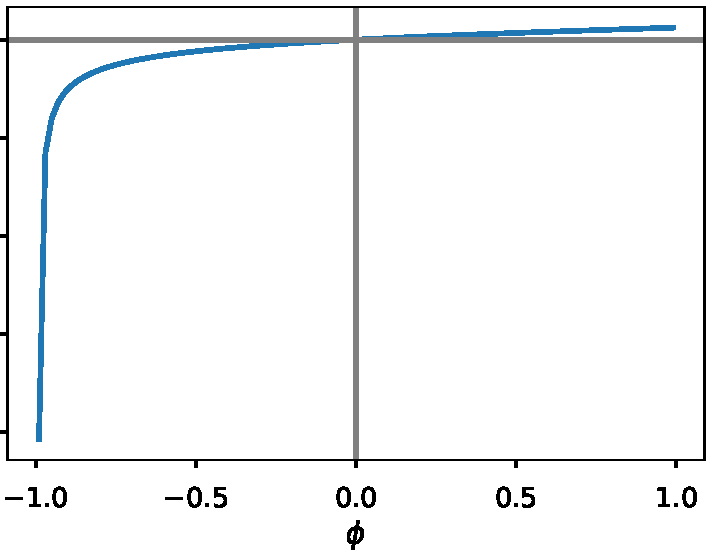
\includegraphics[width=.5\textwidth]{gamma_diff_theta2.pdf}
\end{figure}


\section{Weak Identification Setup}

In this section, take the model described in the previous sections and place it in the setup of
\textcite{andrews2014Gmm} so that we ca analyze the effects of possible lack of identification in the model in a
nice clean way.
The goal here is to perform valid inference for $\pi, \theta$ even when $\phi$ might be zero. 


From the discussion above, we can collect the parameters discussed above into a parameter vector of the following
form,i.e.\@ recall the following: $\eta = \lbrace \rho, c, \delta, \phi, \pi, \theta \rbrace$
To write it in the notation of \textcite{andrews2014Gmm}, we partition $\eta$ into three subsets.

\begin{align}
    \phi &\coloneqq \phi  \in (-1, 1) \\ 
    \zeta &\coloneqq \lbrace \rho, c, \delta, \theta \rbrace \in [0,1) \times \R_{++} \times \R_{++} \times
    \R  \\
    \pi &\coloneqq \pi \in \R 
\end{align}

Let $\Eta$ be the set of possible $\eta$, that as defined above.
It is worth noting that the parameter space has a product form, i.e.\@ the values do not affect the valid values
of the other parameters.

In this environment, $\pi$ is not identified when $\phi = 0$.
Both $\phi$ and $\zeta$ are always identified, and $\zeta$ does not affect the identification of $\pi$.

Let $Q_T(\eta)$ be the GMM criterion function, then the GMM estimator $\hat{\eta}_T$ satisfies the following.


\begin{equation}
    \widehat{\eta}_T \in \Eta\ \text{and}\ Q_T(\hat{\eta}_T) = \inf_{\eta \in \Eta} Q_T(\eta) +
    o\left(T^{-1}\right) 
\end{equation}


Now that we have defined the parameters, we can characterize the set of assumptions necessary for valid inference.
We will work through the assumptions described in \textcite{andrews2014Gmm}.
The set of necessary assumptions is relatively complicated because we have to characterize the asymptotic
distribution under several different estimation strengths simultaneously, and the assumptions required to do that
  differ in the various cases. 
In what follows, we will use 

The first assumption specifies the basic identification
problem. It also provides conditions that are used to determine the
probability limit of the GMM estimator, when it exists, under all categories
of drifting sequences of distributions.
Let $\xi$ index the part of the distribution of the data $r_{t+1}, \sigma^2_{t+1}$ that is not determined by the
moment equations.
In general, it is a (likely infinite-dimensional) nuisance parameter that affects the distribution of the data. 


We collect the parameters that we are estimating $\eta$ and the nuisance parameter $\xi$ into one parameter,
$\gamma$ and associated parameter space $\Gamma$.
In the previous discussion we characterized the parameter spaces in a non-compact fashion, let $\Eta^{*}$ be a
compact subset of $\Eta$, where the true parameter values live.
%TODO Does the set of possible nuisance parameters depend upon the estimated parameters in our model?

\begin{defn}{Complete Parameter Space}
    \begin{equation}
        \Gamma \coloneqq \left\lbrace \gamma = (\eta, \xi) \mvert \eta \in \Eta, \xi \in \Xi \right\rbrace 
    \end{equation}
\end{defn}

We characterize these drifting sequences of distributions by sequences of true parameters $\gamma_T \coloneqq
(\eta_T, \phi_T)$.

\purple{TODO Add discussion of the limiting process.}
\purple{Verify that the assumptions on the parameter space hold.}
\purple{Discuss what happens if we lack identification and hence cannot consistently estimate the parameter.}


\begin{restatable}[Inference for $\eta$ under Weak Identification]{theorem}{InferenceWeakID}
    Let that $\phi_0  \in \left(\underline{\phi}_0,1\right)$, for some $\underline{\phi}_0 > -1$. 
    $\rho_0 \in \left[0,1\right)$, and $c_0 > 0$. 

    \purple{TODO  Add Conclusion}
\end{restatable}


\section{Simulations}

\section{Data}\label{sec:data}

We also assume that $\left[ \frac{\psi}{\phi} \right]^2 \approx \frac{\E \left[\sigma^2_{t+1} \mvert
\F_t\right]}{\Var\left[r_{t+1} \mvert \F_t\right]}$, which enables our approximation of $\sigma^2_{t+1}$ by the
realized volatility.

\section{Empirical Results}

\section{Conclusion}

\clearpage

\phantomsection
\addcontentsline{toc}{section}{References}
\printbibliography
\clearpage

\begin{appendices}


\section{Identification Proofs}

\section{Inference Assumptions}

    In what follows, three sets of drifting sequences $\lbrace \gamma_T \rbrace$ are key. 
    
    \begin{defn}{Drifting Sequence Parameter Spaces}
        \begin{align}
            \Gamma\left(\gamma_0\right) &\coloneqq \left\lbrace \left\lbrace \gamma_T \in \Gamma \right\rbrace
            \mvert \gamma_T \to \gamma_0 \in \Gamma \right\rbrace\\ 
            \Gamma(\gamma_0, 0, b) &\coloneqq \left\lbrace \lbrace \gamma_T \rbrace \in \Gamma(\gamma_0) \mvert
            \phi_0 = 0\ \text{and}\ \sqrt{T} \phi_T \to b \in (\R \cup \lbrace \pm \infty) \right\rbrace \\
            \Gamma(\gamma_0, \infty, b_0) &\coloneqq \left\lbrace \lbrace \gamma_T \rbrace \in \Gamma (\gamma_0)
            \mvert \sqrt{T} \norm{\phi_T} \to \infty\ \text{and}\ \frac{\phi_T}{\norm{\phi_T}} \to b_0
            \right\rbrace 
        \end{align}
    \end{defn}
    
    These are the standard GMM regularity conditions appropriately adjusted for the lack of identification when
    $\phi =0$.
    
    \begin{assump}[GMM 1]\label{ass:GMM1}
    \begin{assumplist}
        \item If $\phi_0=0$, $\sampmom(\eta)$ and $\W_{T}(\eta)$ do not depend on $\pi$ for all $\eta \in \Eta$,
            for all $T \geq 1$, and for all $\gamma^{*}\in \Gamma.$ 
            \label{ass:GMM1a}
        \item If $\lbrace \gamma_{T} \rbrace \in \Gamma\left(\gamma_0\right)$, $\sup_{\eta \in \Eta}
            \norm*{\sampmom(\eta) - \E\left[g\left(\eta \mvert \gamma_0\right)\right]} \pto 0$ and $\sup_{\eta
            \in \Eta} \norm{\W_{T}(\eta)-\E\left[\W\left(\eta \mvert \gamma_0\right)\right]} \pto 0$.
            \label{ass:GMM1b}
        \item When $\phi_0 = 0$,  $g_0\left(\phi, \zeta ,\pi \mvert \gamma_0\right) = 0$ if and only if $\phi
            =\phi_0$ and $\zeta = \zeta_0$ for all $\pi \in \Pi$ and for all $\gamma_0 \in \Gamma.$
            \label{ass:GMM1c}
        \item When $\phi_0 \neq 0$, $g_0\left(\eta \mvert \gamma_0\right)=0$ if and only if $\eta =\eta_0$ for all
            $\gamma_0 \in \Gamma.$
            \label{ass:GMM1d}
        \item  $g_0\left(\eta \mvert \gamma_0\right)$ is continuously differentiable in $\eta $ on $\Eta$ with
            partial derivatives with respect to $\eta$ and $\xi$ denoted by $g_{\eta}\left(\theta \mvert
            \gamma_0\right) \in R^{k\times d_{\eta }}$ and $g_{\xi }\left(\eta \mvert \gamma_0\right)\in R^{k\times
            d_{\xi }}$, respectively.
            \label{ass:GMM1e}
        \item $\W\left(\eta \mvert \gamma_0\right)$ is continuous in $\eta$ on $\Eta$ for all $\gamma_0\in
            \Gamma$.  \label{ass:GMM1f}
        \item $0 < \lambda_{\min}(\W\left(\xi_0, \pi \mvert \gamma_0\right))\leq \lambda_{\max }(\W\left(\xi_0,\pi
            \mvert \gamma_0\right)) < \infty$, $\forall \pi \in \Pi$, for all $\gamma_0 \in \Gamma$.
            \label{ass:GMM1g}
        \item $\lambda_{\min} (g_{\xi}\left(\xi_0,\pi \mvert \gamma_0\right)^{\prime} \W\left(\xi_0,\pi \mvert
            \gamma_0\right)g_{\xi }\left(\xi_0,\pi \mvert \gamma_0\right))>0$, for all $\pi \in \Pi$,  and for all 
            $\gamma_0 \in \Gamma$ with $\phi_0=0.$
            \label{ass:GMM1h}
        \item$\Xi(\pi)$ is compact for all $\pi \in \Pi$, and both $\Pi$ and $\Eta$ are compact.
            \label{ass:GMM1i}
        \item For all $\epsilon > 0$, there exits a $\delta > 0$ such that $d_{H}\left(\Xi \left(\pi_{1}\right),
            \Xi \left( \pi_{2}\right) \right) < \epsilon$ for $\pi_{1}, \pi_{2} \in \Pi$ with
            $\norm*{\pi_{1}-\pi_{2}} < \delta$, where $d_{H}\left( \cdot \right)$ is the Hausdorff metric.
            \label{ass:GMM1j}
    \end{assumplist}
    \end{assump}
    
    
    
    \begin{assump}[GMM 2*]\label{ass:GMM2}
    \begin{assumplist}
        \item $\sampmom(\eta)$ is continuously differentiable in $\eta$ for all $T \geq 1$. 
            \label{ass:GMM2a}
        \item If $\{\gamma_T\} \in \Gamma\left(\gamma_0, 0, b\right)$, $\sup_{\left\lbrace \eta \in \Eta \mvert
            \norm*{(\phi, \zeta')' - (\phi_T, \zeta_0')} \leq \delta_T \right\rbrace}
            \norm*{\frac{\partial}{\partial (\phi, \zeta')'} \sampmom(\eta) - \E\left[\popmom_{(\phi,
            \zeta')'}(\eta) \mvert \gamma_0\right]} = o_p(1)$ for all deterministic sequences  $\delta_T \to 0$.
            \label{ass:GMM2b}
        \item  Let $\Eta_T \coloneqq \left\lbrace \eta \in \Eta \mvert \norm*{(\phi, \zeta_) - (\phi_T, \zeta_T)}
            \leq \delta_T \norm*{\beta_T}\, \text{and}\, \norm*{\pi - \pi_T} \leq \delta_T \right\rbrace$.  Let
            $\delta_T$ be a deterministic sequence that converges to zero.  If $\{\gamma_T \} \in
            \Gamma\left(\gamma_0, \infty, b_0\right)$, then we have the following asymptotic behavior.
            $\sup_{\eta \in \Eta_T} \norm*{\left(\frac{\partial}{\partial \eta'} \overline{g}_T -
            \E\left[g_{\eta}(\eta) \mvert \gamma_0\right]\right) \diag\left(1_{1+d_\zeta}',
            (1/\phi_T)_{d_{\pi}}'\right)}  = o_p(1)$. 
            \label{ass:GMM2c}
    \end{assumplist}
    \end{assump}
    
    Once we have \nameref{ass:GMM1} and \nameref{ass:GMM2}, we use \nameref{ass:GMM3} to derive the asymptotic
    distribution under weak and semi-strong identification.
    These conditions will be characterized using the expected derivative of the population moment conditions. 
    
    \begin{defn}
        \label{defn:moment_derivative_func}
        \begin{equation}
            K_{T,g}\left(\eta \mvert \gamma^{*}\right) \coloneqq  \frac{1}{T} \sum_{i=1}^T \frac{\partial}{\partial
            \phi^{*}} \E \left[ \popmom(W_T, \eta) \mvert \gamma^{*} \right]
        \end{equation}
    \end{defn}
    
    
    \begin{assump}[GMM 3]\label{ass:GMM3}
    \begin{assumplist}
        \item $\sampmom(\eta) = \frac{1}{T} \sum_{i=1}^T \popmom(W_T, \eta)$  for some function $\popmom(W_T,
            \eta) : \R^{k \times k} \times \Eta \to \R^k$.
            \label{ass:GMM3a}
        \item $\E\left[\popmom(W_T, \beta_0, \zeta^{*}, \pi) \mvert \gamma^{*} \right] = 0$ for all $\pi \in \Pi$ and
            for all $i \geq 1$ if $\gamma^{*} = \left(0,\zeta^{*}, \pi^{*}, \xi^{*} \right) \in \Gamma$.
            \label{ass:GMM3b}
        \item If $\{ \gamma_T \} \in \Gamma(\gamma_0, 0, b)$, $\frac{1}{\sqrt{T}} \sum_{i=1}^T \left(g(W_T,
            \zeta_{0,T}, \pi_T) - \E \left[g(W_T, \zeta_{0,T}, \pi_T)\mvert \gamma_T \right]\right)  \dto \N\left(0,
            \aleph(\gamma_0)\right)$, where $\aleph(\gamma_0)$ is a $k \times k$ matrix.
            \label{ass:GMM3c}
        \item 
            \label{ass:GMM3d}
            \begin{enumerate}
                \item  $K_{T,g}\left(\eta \mvert \gamma^{*}\right)$ exists for all $\{\eta, \gamma^{*} \} \in
                    \left(\Eta_{\delta} \times \Gamma_{0}\right)$ and for all $T \geq 1$.
                \item $K_{T,g}\left(\phi_T, \zeta_T, \pi \mvert \widetilde{\gamma}_T\right)$ uniformly converges
                    to some non-stochastic matrix-valued function  $K_{g}\left(0, \zeta_0, \pi \mvert
                    \gamma_0\right)$ over $\pi \in \Pi$ for all deterministic sequences $\{\phi_T, \zeta_T,
                    \widetilde{\gamma}_T \}$ satisfying $\widetilde{\gamma}_T \in \Gamma$, $\widetilde{\gamma}_T
                    \to \gamma_0 \coloneqq (0, \zeta_0, \pi_0, \xi)$, $\{\phi_T, \zeta_T, \pi \} \in \Eta$ and
                    $\{\phi_T, \zeta_T \} \to (0, \zeta_0)$.
                \item $K_g\left(\phi_0, \zeta_0, \pi \mvert \gamma_0\right)$ is continuous on $\Pi$ for all
                    $\gamma_0 \in \Gamma$ with $\phi_0 = 0$.
            \end{enumerate}
            \item $K\left(\phi_0, \zeta_0, \pi \mvert \gamma_0\right) = \popmom_{\phi, \zeta}\left(\phi_0,
                \pi\mvert \gamma_0\right) x$ for some $x \in \R^{1+d_{\zeta}}$ if and only $\pi =
                \pi_0$.\footnote{Since $\dim(\phi) = 1$, we can assume without loss of generality that the
                $\omega_0$ from \textcite{andrews2014Gmm} equals $1$.}
                \label{ass:GMM3e}
            \item If $\{ \gamma_T \} \in \Gamma(\gamma_0, 0, b)$, $\frac{1}{T} \sum_{i=1}^T
                \frac{\partial}{\partial \eta}  \E\left[ \popmom\left(W_T, \eta_T \right ) \mvert \gamma_T \right]
                \to \popmom_{\eta}\left(\eta_0 \mvert \gamma_0\right)$.
            \label{ass:GMM3f}
    \end{assumplist}
    \end{assump}

    \begin{defn}{\popmom*}
        \begin{equation}
            g_{\phi, \zeta}^{*}\left(\phi_0, \zeta_0, \pi_1, \pi_2 \mvert \gamma_0\right)  =
            \left[g_{\phi}\left(\phi_0, \zeta_0, \pi_1 \mvert \gamma_0\right)  , g_{\phi}\left(\phi_0, \zeta_0,
            \pi_2 \mvert \gamma_0\right) , g_{\zeta} \left(\phi_0, \zeta_0 \mvert \gamma_0\right)  \right]  \in
            \R^{k \times (d_{\zeta} + 2)}
        \end{equation}
    \end{defn}


    \begin{assump}[GMM 4]\label{ass:GMM4}
    \begin{assumplist}
        \item $\phi$ is a scalar.
            \label{ass:GMM4a}
        \item $g_{\phi, \zeta}^{*}\left(\phi_0, \zeta_0, \pi_1, \pi_2 \mvert \gamma_0\right)$ has full column
            rank. 
            \label{ass:GMM4b}
        \item $\aleph(\gamma_0)$ is positive definite for all $\gamma_0 \in \gamma $ with $\phi_0 = 0$. 
            \label{ass:GMM4c}
    \end{assumplist}
    \end{assump}

    \section{Inference Proofs}

    \identifiedSet*

    \begin{proof}
    
    Since the exponential function is a strictly positive function, and we are considering a grid of $x$ values, a
    sufficient condition for $\rho, \delta$, \& $c$ to be identified is for the relevant rows of $\nabla a(x)$ and
    $\nabla b(x)$ to equal zero only at $\eta_{0}$ which are satisfied if $\rho, c, \delta > 0$.
    Testing if if $\phi$ and $\theta$ are identified is somewhat trickier. 
    Consider $\nabla \alpha(x)$. 
    Since we are using a grid of $x$'s, and the gradient of $\alpha$ is a nonlinear function of $x$, the first two
    rows of the \cref{eqn:alpha_gradient} imply $\phi$ is identified.
    
    \begin{equation}
        \label{eqn:alpha_gradient}
        \frac{\partial \alpha(x)}{\partial (\phi, \theta, c)'}  = \begin{bmatrix} \phi x^{2} + x \left(- 2 \beta
        \left(\theta_{2} - \frac{1}{2}\right) - \frac{\phi}{2 \sqrt{c} \left(\phi + 1\right)^{\frac{3}{2}}} +
        \frac{1}{\sqrt{c} \sqrt{\phi + 1}}\right) \\ x \left(- \phi^{2} + 1\right) \\ \frac{\phi x}{2
        c^{\frac{3}{2}} \sqrt{\phi + 1}} \end{bmatrix} 
    \end{equation}
    
    The top line of \cref{eqn:alpha_gradient} can be solved for $\theta$, which would create a local lack of
    identification for $\theta$.
    However, this creates a linear relationship between $\theta$ and the other parameters and $x$.
    However, since we are using multiple $x$'s we can avoid this issue.
    Consequently,  $\phi \in (-1,1], c > 0$, are sufficient to identify all of the parameters except for $\pi$,
    the price of volatility risk.
    We can use $a_{\PP}(x)$ to identify $\rho$.
    
    If $\phi = 0$, $\beta(x) = x \left(a (\pi + \alpha(\theta)) - a(\pi + \alpha(\theta))\right)$, and
    $\gamma(x) =  x \left(b (\pi + \alpha(\theta)) - b(\pi + \alpha(\theta))\right)$.
    These both  identically zero, and $\pi$ does not show up in anywhere  else in the criterion function.
    
    \end{proof}


\begin{restatable}[Uniform Convergence under Strong Identification]{lemma}{UllnStrongID}
    \label{lemma:UniformConvergenceStrongID}
    Let $\Eta$ be the identified set defined by \cref{eqn:EtaDefn}.
    Further assume that $\phi_0 \neq 0$. 
    Let $\sampmom$ be the sample moment condition defined above, and $\W_T$ be the associated optimal weight matrix
    estimator.
    Then we have the following convergence.

    \begin{align}
        &\sup_{\eta \in \Eta} \norm*{\sampmom(\eta) - \E\left[g\left(\eta \mvert \gamma_0\right)\right]}_{Fro}
          \pto 0 \\ 
        &\sup_{\eta \in \Eta} \norm{\W_{T}(\eta)-\E\left[\W\left(\eta \mvert \gamma_0\right)\right]} \pto 
    \end{align}

\end{restatable}

\begin{proof}

    In this proof we rely heavily on the continuity of the moment conditions over their domain. 
    This can be seen from simple inspection since we assumed that $\phi_0 \geq \underline{\phi} -1$.
    Furthermore since $\Eta$ is compact, this continuity implies uniform continuity.
    
    For any positive definite weight-matrix by \textcite[Lemma 2.3]{newey1994large} our criterion function has
    a unique optimum.
    The data, $\sigma^2_{t+1}, r_{t+1}$, are ergodic and stationary.
    Since the moment conditions are not redundant the optimal (GMM) weight matrix $\W$ is positive definite. 
    In addition, $\popmom$ is continuous at each $\eta$, given the restrictions above and properties of
    characteristic functions imply that $\popmom$ is uniformly bounded. 
    For convenience, we assume that the space of $\eta$ is compact.
    This should not be an issue here because the parameters  are either a priori bounded, such as $\phi$ or we
    have substantial a priori knowledge on their plausible magnitudes.
    Hence, \textcite[Theroem 2.6]{newey1994large} implies our estimator is consistent.
    
    However, when we allow for weak identification late on, we need this convergence to be uniform. 
    One straightforward way to show this is to show that our criterion function is globally Lipschitz in a set of
    high probability. 
    
    The other issue is that we need the weight matrix to converge uniformly to its expectation.
    Since the moments are continuous functions over their domain as is the square function.
    This convergence is uniform if and only if the matrix inverse is continuous.
    
    Since we have a finite number of non-redundant moments, the minimum eigenvalue, \\
    $\lambda_{min}\left(\W\left(\phi_0, \zeta_0, \pi \mvert \gamma_0\right)\right) > 0$, and so the matrix inverse
    is uniformly continuous in $\gamma_0$ with respect to the Frobenius norm, which is the sum of the eigenvalues.
    (Recall, that the eigenvalues of the inverse are the inverse of the eigenvalues.)


\end{proof}


\begin{assump}[Weak Dependence]
    \label{assumption:weak_dependence}
    $z_t \coloneqq \begin{pmatrix} r_{t+1} \\ \sigma^2_{t+1} \end{pmatrix}$ are $\alpha$-mixing with $\alpha_t =
       O\left(T^{-5}\right)$
\end{assump}


\begin{theorem}[Inference for $\eta$ under Strong Identification]
    Assume that $\phi_0  \in (-1,1) \setminus 0$, $\rho_0 \in [0,1)$, and $c_0 > 0$. 
    Further assume that the data are ergodic, stationary, and satisfy \cref{assumption:weak_dependence}.
    Then the following convergence in distribution holds.

    \begin{equation}
    \sqrt{T} (\widehat{\eta}_T - \eta_0) \dto \N\left(0, \left(G' \E[\W] G\right)^{-1}\right)
    \end{equation}
\end{theorem}

\begin{proof}

    By the above arguments, we have a consistent estimator for $\eta$ and the optimal weight matrix $\W \coloneqq
    (\E\left[g g'\right])^{-1}$, and we will assume that the true value $\eta_{0}$ is in the interior of its
    sample space $\Eta$.\footnote{Throughout we will use subscript \num{0}  to denote true values for parameters.}
    Let $G \coloneqq \E\left[\frac{\partial}{\partial \eta} \popmom \right]$ Clearly, $g$ is continuously
    differentiable, and its derivative $G$ is continuous.
    In addition, by the identification discussion $G' W \nabla G$ is nonsingular.
    
    %TODO Replace this with strong (alpha) mixing of order (1+\epsilon). 
    %Don't you need a lot more than this...?

    Since, $\norm*{g_t}$ is almost surely bounded by $1$ it has all of its moments and $z_t$ being $\alpha$-mixing
    implies $g_t$ is as well by the central limit theorem for strongly mixing process $\sqrt{T} \sampmom(\eta^{*})
    \dto \N\left(0, \E\left[\W\right]^{-1}\right)$ as required. 
    Consequently, by \textcite[theorem 3.2]{newey1994large} we have convergence in distribution as well as
    convergence in probability.
    

\end{proof}


\InferenceWeakID*

\begin{proof}
We prove this result by showing that Assumptions GMM 1-4 are satisfied.

\begin{proofpart}
    \label{part:main_theorem_proof_part1}
    In this part, we show that \nameref{ass:GMM1} is satisfied. 
    To do this, we break \nameref{ass:GMM1}  down into three subsections.
    Assumptions \namedref{ass:GMM1a}, \namedref{ass:GMM1b}, \namedref{ass:GMM1c}, and \namedref{ass:GMM1d} state
    that when $\phi = 0$, the moment conditions contain no information regarding $\pi$, but when $\phi \neq 0$,
    the model is identified.
    This is what we show in \cref{lemma:IdentifiedSet}.
    We further showed the relevant uniform convergence to verity \namedref{ass:GMM1b} in
    \cref{lemma:UniformConvergenceStrongID}.
    
    The next two assumptions (\namedref{ass:GMM1e} and \namedref{ass:GMM1f}) are  technical conditions regarding
    the behavior of the moment conditions and weight matrix. 
    Since our moment conditions are derived from an infinitely-differentiable  characteristic function and the
    weight matrix is the optimal one, they both hold trivially.
    
    The third subsection of Assumption \nameref{ass:GMM1} concerns the weight matrix.
    Since we are using the inverse covariance matrix of valid non-redundant model, assumptions
    \namedref{ass:GMM1g} and \namedref{ass:GMM1h} automatically hold.
    
    The last two assumptions, \namedref{ass:GMM1i} and \namedref{ass:GMM1j} require that the parameter spaces do
    not vary too much with the parameters and are compact.
    Since $\Eta$ is compact, \namedref{ass:GMM1i} holds trivially, and since it has  has a product form,
    \namedref{ass:GMM1j}  holds trivially as well.
    
\end{proofpart}


\begin{proofpart}
    \label{part:mainTheoremProofPart2}

    In this section, we show that the derivatives of the moment conditions have the correct behavior locally to
    the true parameters.
    We have to do this for the different classes of drifting sequences.
    We will do this by verifitying \cref{ass:GMM2}.
    This is valid since \textcite{andrews2014Gmm} show that this is a sufficient condition for their Assumption
    GMM2, which is what we actually need. 

    Our moment conditions are sample averages of the characteristic function, they satisfy \namedref{ass:GMM2a}
    automatically. 
    Since characteristic functions are uniformly bounded, by the dominated convergence theorem we can interchange the 
    expectation and derivative operators. 
    Hence \namedref{ass:GMM2b} and \namedref{ass:GMM2c} are equivalent to the statements in terms of the moment
    conditions themselves mutatis mutandis.  
    In addition, sice the derivate is a linear operator, we can pull it outside of the norm.
    The reason that the uniform law of large numbers in \cref{part:main_theorem_proof_part1} does not trivially
    imply this result is because we are not considering sequences $\phi_T \to \phi_0$. 


    We create a mean value expansions around around $(\phi_0, \zeta_T, \pi_T)$ of the sample moment condition and
    around $(\phi_0, \zeta_0, \pi_0)$ for the population moment condition.
    (This is not the same in both cases, not is it the true parameter for the drifting sequence in the case of the
    sample moment condition.)
    In addition, also since we are considering continuous functions of compact spaces --- the $\delta_T$ ball in
    $\R^{\dim(\eta)}$ --- pointwise convergence implies uniform convergence, and so we only need to show pointwise
    convergence below.

    \begin{alignat}{2}
        & &&\norm*{\sampmom(\phi_T, \zeta_T, \pi_T) -  \E\left[\popmom(\phi_T, \zeta_T, \pi_T) \mvert
          \gamma_0\right] } \\ 
        \intertext{We take a mean value expansion of both functions around $\eta_0$. The point at which the
        derivative in the two locations is taken may not be the same.}
        &= &&\left\lVert \sampmom(\phi_0, \zeta_0, \pi_0) + \frac{\partial}{\partial (\phi, \zeta,
           \pi)}\sampmom(\widetilde{\phi}^s, \widetilde{\zeta}^s, \widetilde{\pi}^s)\left((\phi_0, \zeta_0, \pi_0)
            - (\phi, \zeta, \pi)\right)\right. \\
        &  &&\quad \left. - \E\left[\popmom(\phi_0, \zeta_0, \pi_0) \mvert \gamma_0\right] + 
           \frac{\partial}{\partial (\phi, \zeta, \pi)} \E\left[\popmom(\widetilde{\phi}^p, \widetilde{\zeta}^p,
           \widetilde{\pi}^p)\mvert \gamma_0\right] \left((\phi_0, \zeta_0, \pi_0) - (\phi, \zeta,
           \pi)\right) \right\rVert \\ 
        \intertext{By the triangle inequality.}
        &\leq && \norm*{\sampmom(\phi_0, \zeta_0, \pi_0) - \E\left[\popmom(\phi_0, \zeta_0, \pi_0) \mvert
           \gamma_0\right]}  \\
        &+  && \norm*{\frac{\partial}{\partial (\phi, \zeta)}\sampmom(\widetilde{\phi}^s, \widetilde{\zeta}^s,
          \widetilde{\pi}^s)\left((\phi_0, \zeta_0)  - (\phi, \zeta)\right) -  \frac{\partial}{\partial (\phi,
          \zeta)} \E\left[\popmom(\widetilde{\phi}^s, \widetilde{\zeta}^p, \widetilde{\pi}^p)\mvert \gamma_0\right]
          \left((\phi_0, \zeta_0) - (\phi, \zeta)\right)} \\
        &+  && \norm*{\frac{\partial}{\partial \pi}\sampmom(\widetilde{\phi}^s, \widetilde{\zeta}^s,
          \widetilde{\pi}^s)\left(\pi_0 - \pi\right) -  \frac{\partial}{\partial \pi}
          \E\left[\popmom(\widetilde{\phi}^p, \widetilde{\zeta}^p, \widetilde{\pi}^p)\mvert \gamma_0\right]
          \left(\pi_0 - \pi\right)} 
          \label{eqn:pi_derivative_term}
    \end{alignat}

    By the uniform law of law numbers in \cref{part:main_theorem_proof_part1}, the first equation is $o_p(1)$.
    For $(\phi_0, \zeta_0) - (\phi, \zeta)$ small, the middle term is bounded by the quantity below. 


    \begin{equation}
        \norm*{\frac{\partial}{\partial (\phi, \zeta)}\sampmom(\widetilde{\phi}^s, \widetilde{\zeta}^s,
        \widetilde{\pi}^s) -  \frac{\partial}{\partial (\phi, \zeta)} \E\left[\popmom(\widetilde{\phi}^s,
        \widetilde{\zeta}^p, \widetilde{\pi}^p)\mvert \gamma_0\right]} \norm*{(\phi_0, \zeta_0) - (\phi, \zeta)}
    \end{equation}

    The first term is almost surely bounded, and the second term is less than $\delta_T$ by assumption, and so the
    product is $o_p(1)$.

    The hard part is the third expression.
    Like before we can bound the pull the $\pi_0 - \pi$ term out of the equation.
    However, this term is no longer converges to zero.
    We will consider the two cases, separately.
    Throughout, we will refer to the behavior of the following equation, which bounds
    \cref{eqn:pi_derivative_term}.


    \begin{equation}
        \norm*{\frac{\partial}{\partial \pi}\sampmom(\widetilde{\phi}^s, \widetilde{\zeta}^s, \widetilde{\pi}^s) -
        \frac{\partial}{\partial \pi} \E\left[\popmom(\widetilde{\phi}^p, \widetilde{\zeta}^p,
        \widetilde{\pi}^p)\mvert \gamma_0\right] } \norm*{\pi_0 - \pi} 
        \label{eqn:pi_derivative_norm_bound}
    \end{equation}

    In general, $\tilde{\pi}^s$ and $\tilde{\pi}^p$ can be arbitrarily far apart.
    However, since $\sampmom \pto \E\left[\popmom \mvert \gamma_0\right]$, and the limiting value is independent of
    $\pi$, the derivative does not depend upon $\pi$ asymptotically by the dominated convergence theorem.
    This applies that the difference between the two derivatives evaluated at different $\pi$ converges to zero.
    Consequently, \cref{eqn:pi_derivative_norm_bound} is $o_p(1)$ and we have shown \namedref{ass:GMM2b}.

    \begin{equation}
        \norm*{\abs*{\frac{\partial}{\partial \pi}\sampmom(\widetilde{\phi}^s, \widetilde{\zeta}^s,
        \widetilde{\pi}^s) - \frac{\partial}{\partial \pi} \E\left[\popmom(\widetilde{\phi}^p,
        \widetilde{\zeta}^p, \widetilde{\pi}^p)\mvert \gamma_0\right]} (1, 1, T)} \norm*{\pi_0 - \pi} 
        \label{eqn:pi_derivative_rescaled_bound}
    \end{equation}

    If we consider the setup in \namedref{ass:GMM2c}, $\tilde{\pi}^s$ and $\tilde{\pi}^p$ are now close together.
    However, we need to show that \cref{eqn:pi_derivative_rescaled_bound} is $o_p(1)$.
    Since we are considering the limiting behavior of a function with a continuous derivative, we can assume that
    the derivative is uniformly bounded without loss of generality. 
    (The constant might depend upon the true value, but not $T$.)
    By a Taylor series expansion of $\sampmom$ around the true value, $\frac{\widetilde{\pi}^p}{\sqrt{T}} \to 0$,
    and $\norm{\pi_0 - \pi} \propto \delta_T$ the result follows.

\end{proofpart}

\begin{proofpart}
    \label{part:mainTheoremProofPart3}

    Assumption \namedref{ass:GMM3a} is trivially satisfied,  and we showed that \namedref{ass:GMM3b} is satisfied
    in \cref{sec:GMM}.  
        
    The conceptual idea driving the reulsts this section is that moment conditions for each $T$ minus their
    conditional exceptions converge to a normal random variable.
    In other words, we are almost in a standard triangular C.L.T.\@ setup with weak time-dependence.

    In particular, both $\sigma^2_t$ and $r_t$ are infinitely differentiable functions of the innovations to
    the volatility and return processes and $\popmom$ are infinitely differentiable functions of $r_{t+1}$ and
    $r_t$ and the innovations are i.i.d.\@ across time by assumption.
    (Note, i.i.d.\@ implies strong mixing of any size.)
    Consequently, $\popmom$ is near epoch dependent (NED) of any size as defined in
    \textcite{andrews1991empirical}.  
    (Take $s>2.$) 
    By \textcite[Theorem 3]{andrews1991empirical}, we have the necessary finite-dimensional convergence in
    distribution to a Gaussian random variable. 

    We now show that \namedref{ass:GMM3d} holds.
    Clearly, $K_{t,g}\left(\eta \mvert \gamma^{*}\right)$ always exists.
    It uniformly converges because the derivatives of the moments are continuous functions of the data and the
    parameters, the process is ergodic, and the characteristic function lives on a compact set.
    It is also clearly continuous.
    By the dominated convergence theorem, we can exchange the derivative and expectations.
    In addition, since \popmom\ does not depend upon $\phi_T$, the limiting behavior is independent of the value
    of $\phi_T$.
    Hence \namedref{ass:GMM1d} holds.
    
    \namedref{ass:GMM3e} says the derivative of the moment function does not depend the true parameter $\phi$ if
    and only if  $\pi =  \pi_0$. 
    We showed this in the proof of \cref{part:mainTheoremProofPart2}.
    \namedref{ass:GMM3f} follows directly from the compactness of the parameter space and the continuity of the
    cross derivatives of \popmom\ by the dominated convergence theorem.

\end{proofpart}

\begin{proofpart}
    \label{mainTheoremProofPart4}
   
    \namedref{ass:GMM4a} holds trivially.
    We verified \namedref{ass:GMM4b} when we showed that $\pi$ and $\zeta$ are strongly identified
    (\cref{lemma:IdentifiedSet}).
    \namedref{ass:GMM4c} holds because the identification conditions do not create any singularity in the
    asymptotic covariance matrix. 

\end{proofpart}

\end{proof}





\end{appendices}


\end{document}


